
From the previous investigation it is clear
that it is not possible to incorporate the
hydrogen energy directly \ldots. In the
real system the electrons would move
between states at a much shorter time
period than that of hydrogen tunnelling.
After an electron transitions to a lower
band the fermi distribution should therefore
be recovered almost instantaneously.
The tunneling rate ignoring the
hydrogen energy difference should
therefore provide a good approximation
for the true tunneling rate, as the
electron should only spend a small
fraction of it's time in the lower band.

\subsection{}
To calculate the overall tunneling rate
the simulation was repeated in small
bands (of width cite TODO)




\subsection{Degenerate Tunnelling at 150K}
The tunnelling was simulated at various occupancy,
however the rate was seen to change as the
number of electrons was increased.

and the rate curve was fitted to
\begin{equation}
    R(N,N) = 4 R_0 N(1-N)\label{eqn:degenerate tunnelling rate}
\end{equation}

\subsection{Calculating \(R_0\)}
Since the rate depends only on a single
parameter \(R_0\) we are able to
extrapolate the rate at all
occupancy from the asymptotic
limit of the rate at a single
occupation fraction. This can
only be achieved for
\(N=\frac{1}{2}\), where
by far the largest number of
datapoints were collected (TODO-PLOT).
We are also able to extrapolate
\(R_0\) from the asymptotic
rates for states with n electrons.
As \(N\rightarrow{}0\)
we find
\(R(N,N) \sim{} 4 R_0 N = 4R_0 (\frac{n}{s})\).
We are therefore able to
use the gradient as the
number of states \(s\rightarrow{}\infty{}\)
to find \(R_0\).
Since the rate curve
is symmetric we expect
identical behaviour for
n holes, however
since the 1 electron
data was inconsistent (TODO cite)
we limit the analysis to 2 electron
or 2 hole data.

The calculated rate constants
are given in \cref{tab:extracted rate constant}.
\begin{table}[htbp]
    \begin{center}
        \begin{tabular}{ *{2}{c} }
            \toprule
            Filling                 & \(R_0\)                    \\
            \midrule
            \(\frac{1}{2}\) Filling & \(\mathcal{O}(n^3 + n d)\) \\
            \(2\) Electron Rate     & \(\mathcal{O}(n^2 + n d)\) \\
            \bottomrule
        \end{tabular}
    \end{center}
    \caption{Extracted value of \(R_0\) from the
        simulated rate for half filled
        states and two electron states.
    }\label{tab:extracted rate constant}
\end{table}

\subsection{Correcting for Reversed Rate}
When we attempted to include hydrogen
energy in \cref{sec:different hydrogen energy}
we found electron tunneling between states
degenerate in energy. We should therefore
correct the tunneling rate accordingly.
Due to
the arguments outlined in
\cref{app:combined tunnelling rates}
a general system with a different
forward and backward rate has a combined rate
\begin{equation}
    R(N,N') = R(N\rightarrow{}N') + R(N'\rightarrow{}N)
\end{equation}
where \(R(N\rightarrow{}N')\) is the
tunneling rate from an occupation \(N\)
to an occupation \(N'\). From
\cref{eqn:degenerate tunnelling rate}
it is clear that
\begin{equation}
    R(N\rightarrow{}N) = 2R_0N(1-N)
\end{equation}
By requiring the correct
behaviour at \(N' = N\), there are
three ways to modify the tunneling
rate
\begin{align}
    R(N\rightarrow{}N') & = 2R_0N(1-N)                 \\
    R(N\rightarrow{}N') & = 2R_0N(1-N')                \\
    R(N\rightarrow{}N') & = 2R_0 \sqrt{N(1-N)N'(1-N')}
\end{align}
note we have ignored functions
such as \(2R_0N'(1-N')\) which
would give the same overall rate
as \(2R_0N(1-N)\).

\subsection{Total Tunnelling Rate}
To recover the total tunneling
rate the occupation rate curve
is converted into an
energy rate using the
fermi-dirac distribution (TODO cite).
For example for \(R(N\rightarrow{}N') = 2R_0N(1-N')\)
we find
\begin{align}
    N(\epsilon)             & = \frac{1}{1 + \exp{(\beta(\epsilon - \mu))}}                                                                         \\
    R(\epsilon-> \epsilon') & = 2R_0 \frac{1}{1 + \exp{(\beta(\epsilon - \mu))}}(1- \frac{1}{1 + \exp{(\beta(\epsilon' - \mu))}})                   \\
                            & = 2R_0 \frac{\exp{(\beta(\epsilon' - \mu))}}{(1 + \exp{(\beta(\epsilon - \mu))})(1 + \exp{(\beta(\epsilon' - \mu))})}
\end{align}
where we have assumed uniform
occupation within a band.
The rate curve
(\cref{fig:tunneling rate against energy})
can then be
integrated to give an
overall tunneling rate.
\begin{figure}[htbp]
    \centering
    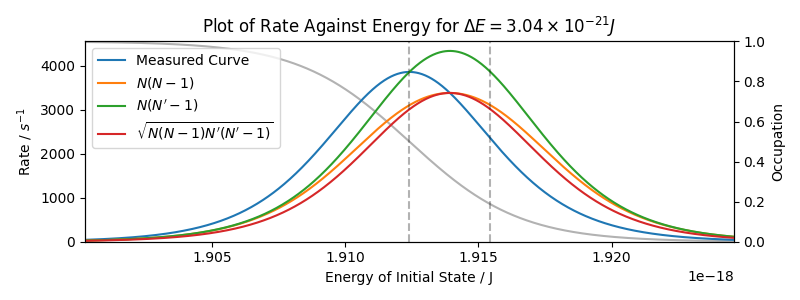
\includegraphics[width =0.9 \linewidth]{Figures/Simulation/Corrected Decay Rates.png}
    \caption{Plot of the corrected
        tunneling rate curve against
        energy. As the occupation curve
        (shown in grey) falls to 0
        the rate falls also. The corrected
        rate is seen to peak at half of the hydrogen
        energy difference above the fermi
        energy (grey dashed line).
    }\label{fig:tunneling rate against energy}
\end{figure}

TODO-No temp dependence seen in
initial rate data
\subsection{Investigating Rate Corrections}
Given the calculated tunneling rates
it is possible to compare
the temperature dependence
with experiment. In (TODO-fig)
we find that all

We do however see much smoother
behaviour as \(T\rightarrow0\)
with the choice \(\sqrt{}\),
suggesting it could be the most
physically justifies. The tunneling rate
implied
by the 2 electron data
is however slightly larger
than measured in experiment (TODO-fig)



\subsection{Tunneling without Self Interaction}
\ldots only introduce an offset in energy
we might be tempted to exclude this self interaction

the tunnelling rate is however much different
in this case





\subsection{Simulation With Multiple Spins}


\subsection{Bosons with Constrained Occupation}
To investigate the effect of fermion spin
statistics \ldots to calculate the rate
for bosons.
